% DO NOT COMPILE THIS FILE DIRECTLY!
% This is included by the other .tex files.




%\section{Gibbs sampling for a hierarchical normal model} 
%
%\begin{frame}{Goal}
%	
%In the context of Bayesian inference, we show an example in which Gibbs sampling is the natural choice, since conditional posteriors are available (and simple).\\
%\vspace{0.2in}
%The bayesian analysis is taken from:\\
%Gelman, A., Carlin, J. B., Stern, H. S., Dunson, D. B., Vehtari, A., \& Rubin, D. B. (2014).\textit{ Bayesian data analysis (Vol. 2)}. %Boca Raton, FL: 
%CRC press.
%
%\end{frame}
%
%
%\begin{frame}{The data}
%
%Coagulation time in seconds for blood drawn from 24 animals randomly allocated to four different diets.\\
%
%\begin{figure}
%	\centering
%	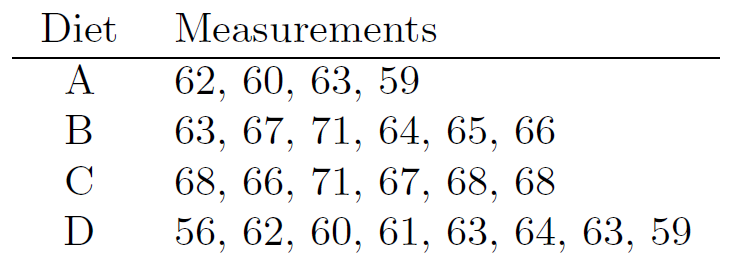
\includegraphics[width=0.7\columnwidth]{images/hier_data.png}
%\end{figure}
%
%From Box, G. E., Hunter, W. G., \& Hunter, J. S. (1978). \textit{Statistics for experimenters: an introduction to design, data analysis, and model building (Vol. 1)}. New York: Wiley.
%
%\end{frame}
%
%
%\begin{frame}{Model, prior and joint posterior}
%
%Hierarchical model:
%\begin{align*}
%y_{ij} \mid \theta, \sigma &\sim N(\theta_j,\sigma^2) \quad \quad \quad i=1, \ldots, n_j \quad \quad  j=1,\ldots, J \\
%\theta_j \mid \mu, \tau &\sim N(\mu,\tau^2) \\
%\end{align*}
%
%Prior:\\
%\vspace{0.1in}
%$\quad \quad p(\mu, \log\sigma, \log\tau) \propto \tau $\\
%\vspace{0.2in}
%Joint posterior:\\
%\vspace{0.1in}
%$\displaystyle p(\theta,\mu,\log\sigma,\log\tau \mid y) \propto \tau \prod_{j=1}^J N(\theta_j \mid \mu,\tau^2) \prod_{j=1}^{J} \prod_{i=1}^{n_j} N(y_{ij} \mid \theta_j,\sigma^2)$
%
%\end{frame}
%
%
%\begin{frame}{Conditional posteriors}
%
%$\theta_j \mid \mu, \sigma, \tau, y \sim N  \left( \hat{\theta_j},V_{\theta_j} \right)  \quad \mbox{where} \quad \hat{\theta_j} = { {{1 \over \tau^2} \mu + {n_j \over \sigma^2} \bar{y}_{\cdot j} } \over {{1 \over \tau^2}+{n_j \over \sigma^2}}}, \quad V_{\theta_j}= { 1 \over {{1 \over \tau^2}+{n_j \over \sigma^2}}} $ \\
%
%$ \displaystyle \mu \mid \theta, \sigma, \tau, y \sim N \left( \hat{\mu},{\tau^2 \over J} \right) \quad \mbox{where} \quad \hat{\mu} = {1 \over J} \sum_{j=1}^{J} \theta_j $ \\
%
%$ \displaystyle \sigma^2 \mid \theta, \mu, \tau, y \sim Inv.\chi^2 \left( n,\hat{\sigma}^2 \right)  \quad \mbox{where} \quad \hat{\sigma}^2 = {1 \over n} \sum_{j=1}^{J} \sum_{i=1}^{n_j} (y_{ij}-\theta_j)^2 $ \\
%
%$ \displaystyle \tau^2 \mid \theta, \mu, \sigma, y \sim Inv.\chi^2 \left( J-1,\hat{\tau}^2 \right)  \quad \mbox{where} \quad \hat{\tau}^2 = {1 \over {J-1}} \sum_{j=1}^{J} (\theta_j-\mu)^2 $
%
%\end{frame}
%


\section{Independent MH for the mixture of two normal distributions}


\begin{frame}{The model}

The model is a mixture of two normals with fixed parameters\\
$$\mu_1=7, \quad \mu_2=10, \quad \sigma_1=\sigma_2=0.5$$
and unknown (random) mixing proportion $\delta$.\\
\vspace{.1in}
Hence the model is:
$$ y_1, \ldots, y_n \mid \delta \quad \overset{i.i.d.}{\sim} \quad \delta N(\mu_1,\sigma_1^2) + (1-\delta) N(\mu_2,\sigma_2^2)$$\\
\vspace{0.2in}
We generate a sample of size $n=100$ with $\delta=0.7$.\\
\vspace{0.1in}
We then sample from the posterior for $\delta$ with an \textbf{independent MH} using the prior as proposal distribution.\\
\vspace{0.1in}
We expect the posterior to concentrate around the ``true" value $\delta=0.7$.
 
\end{frame}


\begin{frame}{Recall: Metropolis-Hastings (MH)}
	
		\begin{enumerate}
		\item \textbf{Initialization:} Set $t=0$ and sample $x_0$ from a starting distribution
		\item \textbf{At (t+1)-th iteration:} 
			\begin{itemize}
				\item sample the candidate $x^*$ from the proposal distribution $g(\cdot \mid x_t)$
				and compute the MH ratio
				$$ R(x_t,x^*) = \frac{f(x^*)g(x_t \mid x^*)}{f(x_t)g(x^* \mid x_t)}$$
				\item sample $u \sim U(0,1)$
				\item if $u < R(x_t,x^*)$ accept $x^*$ as $x_{t+1}$
				\item else set $x_{t+1}=x_t$
			\end{itemize}
		\end{enumerate}
	
	If $g(\cdot \mid x_t) =  g(\cdot)$, we have \textit{independent MH}.\\
	\vspace{.1in}
\textbf{Here:} f = posterior, g = prior $\implies$ R = likelihood ratio.
	
\end{frame}

\begin{frame}{Results: sample paths}

We experimented with a $Beta(1,1)=U(0,1)$ and a more skewed $Beta(2,10)$ as priors. The start was fixed at $\delta_0=0.5$ for both.
\begin{figure}
	\centering
	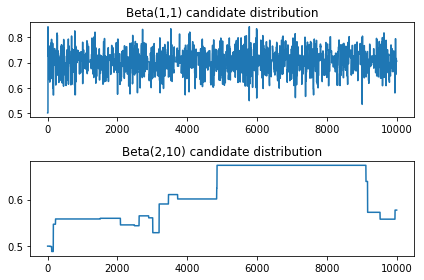
\includegraphics[width=0.5\columnwidth]{images/MCMC_chains.png}
\end{figure}
With the uniform prior, the chain moves away from $\delta_0$ quickly and explores the posterior support well (\textit{good mixing}).\\
\vspace{.1in}
With the $Beta(2,10)$ prior, only a few unique values are accepted and the mixing is poor.

\end{frame}

\begin{frame}{Results: histograms}
	
	We excluded the first 5000 iterations (\textit{burn-in}).
	\begin{figure}
		\centering
		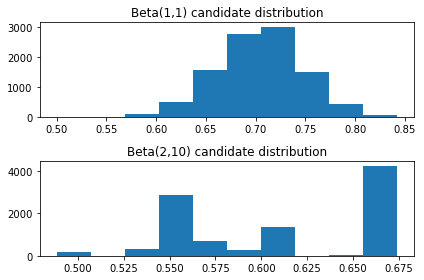
\includegraphics[width=0.5\columnwidth]{images/MCMC_hist.png}
	\end{figure}
	With the uniform prior, we get a sample with posterior mean approximately equal to 0.7, the value we used to generate the data.\\
	\vspace{.1in}
	With the $Beta(2,10)$ prior, we have already seen that we get a lot of ties and the posterior approximation is not reliable.
	
\end{frame}

